\capitulo{3}{Conceptos teóricos}

La parte del proyecto más importante es el proceso de lanzar una aplicación Android desde cero, para ello se ha tenido que realizar una investigación para determinar que herramientas, lenguajes de programación, entornos de desarrollo son los más apropiados para un despliegue ágil.

Todo esto se sitúa en un mercado altamente competitivo, con una gran variabilidad (usuarios, empresas, desarrolladores ...) y con un constante cambio. 

\section{Framework}
Un framework (de origen anglosajón, marco de trabajo), según lo que dice la wikipedia~\cite{wiki:framework}, es una estructura conceptual y tecnológica de soporte definido, normalmente por módulos de software concretos, que sirve de base para la organización y el desarrollo de software. Las ventajas que ofrece son varias, entre las que se puede destacar:

\begin{itemize}
	\item \textbf{Evita repetición de código:} las partes más usadas, pasan a ser algo del \emph{core} del framework.
	\item \textbf{Uso de buenas prácticas:} muchos de estos están basados en patrones de diseño que nos obligan a usar.
	\item \textbf{Elementos avanzados integrados:} cosas complejas y que implementarlas llevaría mucho tiempo, suelen venir integradas.
	\item \textbf{Desarrollo ágil:} por los factores anteriores, podemos centrarnos más en la lógica de negocio de la aplicación que se desea hacer, de una manera más rápida y segura.
\end{itemize}

Por lo tanto, es necesario trabajar mediante frameworks, ya que nos garantizar una aplicación de mayor calidad, que si la hacemos desde cero, en código nativo.

\subsection{Opciones disponibles}
En el mercado existen muchos frameworks disponibles para el desarrollo de aplicaciones móviles, por lo que decantarse por uno no es tarea sencilla, ya que como se aprecia cada uno tiene sus pros y contras. En una encuesta realizada en un foro ~\cite{foro:encuesta}, a mediados del 2019, la opinión de los más recomendados era~\ref{fig:encuesta}:

\begin{figure}[h]
	\centering
	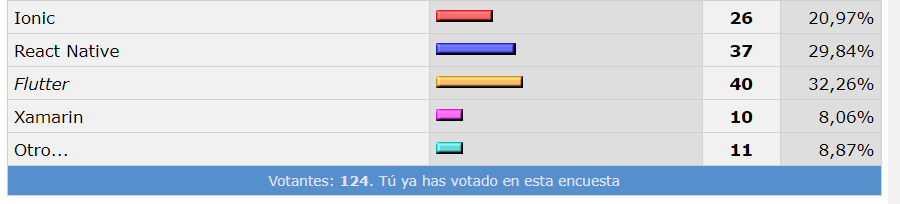
\includegraphics[width=1\textwidth]{teoria/encuesta.png}
	\caption{Encuesta}\label{fig:encuesta}
\end{figure}

Algo ideal es que se intento buscar un framework \emph{crossplataform}, con el que abarcar un mayor mercado, a nivel de usuarios y dispositivos.

\subsubsection{Ionic}
Ionic~\cite{wiki:ionnic} se basa en lenguaje de programación javascript, html y css. Internamente esta basado en otro framework, como es Angularjs. La licencia Open source, fue lanzado en el 2013, permite el desarrollo para iOS y Android. A sufrido gran cantidad de cambios desde entonces.

Ventajas:
\begin{itemize}
	\item Una amplia comunidad de usuarios.
	\item Documentación extensa y de calidad.
\end{itemize}

Algunas de las desventajas:
\begin{itemize}
	\item Rendimiento algo menor, ya que no se desarrolla de forma nativa.
	\item Bibliotecas en constante cambio y evolución, más que ser algo bueno, puede que deje a la aplicación fuera de versión y se tenga que hacer desde cero.
\end{itemize}

\subsubsection{React native}
React native~\cite{wiki:react} fue creado en 2015, de la mano de Facebook. La licencia que tiene es MIT. La diferencia que tiene con React, es que no manipula el DOM, por lo que tampoco usa HTML o CSS. 
Se programa en javascript. Las aplicaciones más conocidas que usan este framework es instgram o facebook.

Ventajas:
\begin{itemize}
	\item Gran comunidad de usuarios y herramientas.
	\item Mejora de las funcionalidades constantemente.
\end{itemize}

Algunas de las desventajas:
\begin{itemize}
	\item Rendimiento algo menor.
	\item No es código nativo, pero casi, por lo que no tiene soporte oficial de Google y Apple.
\end{itemize}

\subsubsection{Xamarin}
Xamarin~\cite{wiki:xamarin} creado por Microsoft en el 2011, por lo que está desarrollado en .NET, siendo propietario.

Ventajas:
\begin{itemize}
	\item Permite el desarrollo de iOS, Android, web pero nativas de escritorio también.
	\item Puede llamar a fragmentos de código usados en otras plataformas.
	\item Soporte para wearables.
\end{itemize}

Algunas de las desventajas:
\begin{itemize}
	\item Acceso limitado a las bibliotecas.
	\item Soporte y actualizaciones lento / tarde.
	\item Comunidad grande pero pequeña comparada con otras.
	\item Aplicaciones de mayor tamaño.
	\item Coste.
\end{itemize}

\subsubsection{Otros}
Hay muchos otros, como kotlin, Apache Cordoba, jQuery Mobile, Native script ...
Pero no me convencieron por diversas razones.
 
\section{Flutter}
Flutter~\cite{wiki:flutter} es un SDK de código abierto creado por Google a finales del 2018. Permite que los desarrolladores puedan crear aplicaciones para iOS, Android y web.

Este se encuentra escrito en Dart, que es un lenguaje de programación creado por Google en 2011. Este lo que hace es una mejora del lenguaje javascript, pero sin pretender sustituirlo. Es decir, ofrecer mejores resultados y alternativas para algunos problemas, siendo una herramienta mejor, para proyectos más grandes, como es el caso de flutter.

Por lo tanto Flutter es una herramienta mi nueva, con la que se pueden hacer aplicaciones comerciales para varias plataformas sin tener que programar exclusivamente para cada una de ellas. Ya que nos ofrece la compilación nativa directamente, reduciendo los costes a la hora de tener que llevar proyectos en los que sea necesario estar en los dos mercados.

Las características más importantes son : 

\begin{itemize}
	\item Desarrollo rápido de las aplicaciones. Cuando se dice rápido es porque permite \emph{hot reload}, esta es la carga en caliente durante la fase de desarrollo. Implica que nos es necesario tener que compilar todo el código, si no aquellas partes que fueron modificadas. Lo que permite en tiempo de ejecución ver los cambios.
	\item Está muy optimizado, con una evolución y soporte constante.
	\item Es un lenguaje de programación respaldado por Google, con lo que esto conlleva. Seguridad, confianza, fiabilidad, soporte, cursos y un montón de herramientas(más de 300 apis distintas: mapas, reconocimiento facial, traductor ... ).
	\item La integración con el sistema operativo Android es mucho más eficaz, ya que este también pertenece a Google.
	\item Cuando se compila, lo hace a nativo, siendo una ganancia de rendimiento.
	\item La curva de aprendizaje es baja, en el caso de que sepamos javascript, typescript o ecmascript.
	\item La calidad de las animaciones.
\end{itemize}

Las desventajas que tiene son:
\begin{itemize}
	\item La mayor parte de la documentación se encuentra en inglés, pero es más problema de desarrollador, que de la propia documentación del framework.
	\item Las aplicaciones ocupan más espacio que las nativas, ya que suelen incluir el SDK al completo.
	\item Al ser tan nuevo, tiene algunos problemas, no ofrece todas las funcionalidades, como las que ofrecen otras plataformas. Google lo sabe y está apostando mucho por ello.
	\item Es una comunidad pequeña, pero a crecido en dos años más que otras, en tiempos similares.
\end{itemize}

Al final me decanto por este Framework básicamente porque es algo nuevo y disruptivo. El respaldo de Google se me presentaba como garantía, con la tranquilidad que eso conlleva. Es decir, todo el \emph{cloud services de Google} se puede integrar con gran facilidad.
Otra de las cosas que fueron de agrado es que la comunidad lo a recibido con los brazos abiertos, como se puede ver en la encuesta~\ref{fig:encuesta}, se encuentra entre los favoritos de los desarolladores, por algo será.

\subsection{Firebase}
Firebase~\cite{wiki:firebase} es una plataforma para el desarollo de apliaciones web, Android e iOS, creada por Google en el 2014. Esta en la nube, formando el \emph{Google Cloud Plataform}, que consta de un conjunto de herramientas para dotar de una calidad enorme a los proyectos. Ya que permite la integración del ecosistema de Google como un todo.

Fue integrada en el proyecto por el hecho de ser un servicio gratuito y que aportaba gran valor a la aplicación. Este pasa a ser de pago cuando la app tiene que escalarse a un nivel más grande, por el tema de usuarios o el número de peticiones que se realicen a la misma. Algunas de las herramientas que integra son de pago, otras no.

Por lo tanto al ser multiplatafomra es un backend con el que poder controlar todo, ganancias, gastos, escalabilidad, nuevos productos, herramientas ... 

Entre los servicios que ofrece tenemos:

\begin{itemize}
	\item \textbf{Real Time Data Base:} base de datos simples en tiempo real, si fuera necesario tener que guardar música, video o fotos, tiene otra parte que es la de Storage.
	\item \textbf{Crash reporting:} herramienta para el reporte de errores que se producen en la aplicación.
	\item \textbf{Autentication:} integración con la mayor cantidad de aplicaciones de redes sociales en las que su API permite esto. Obviamente la propia Google es una de ellas. Lo podemos ver en la siguiente imagen~\ref{fig:inicio}:
	\begin{figure}[h]
		\centering
		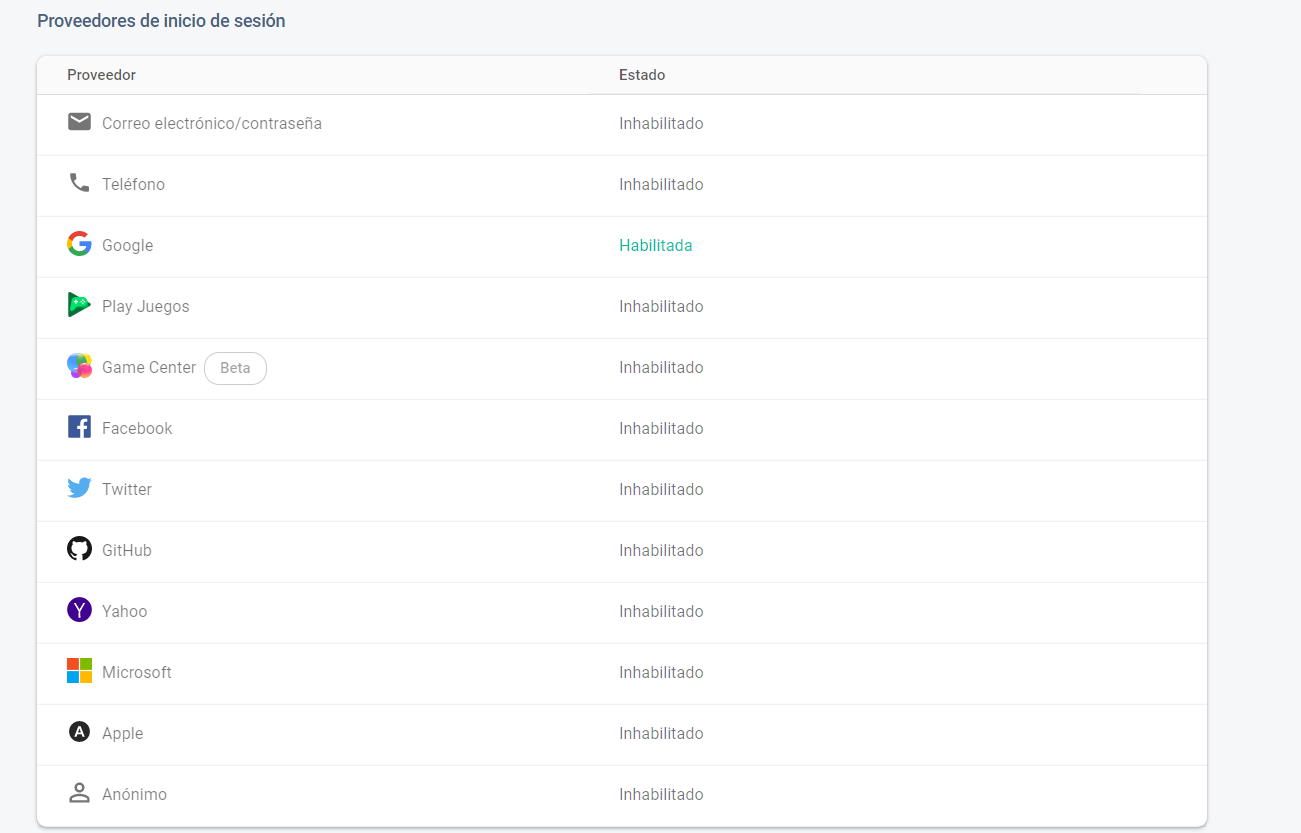
\includegraphics[width=1\textwidth]{teoria/inicio.png}
		\caption{Inicio de sesión}\label{fig:inicio}
	\end{figure}
	\item \textbf{Test lab:} probar la aplicación antes de realizar el despliegue de la misma.
	\item \textbf{Remote config:} hacer cambios internos del funcionamiento de la aplicación sin tener que recomplilar o actualizarla.
	\item \textbf{Hosting:} servidor donde podemos publicar una página web.
	\item \textbf{Análisis:} mediante las analíticas que ofrece~\ref{fig:numerousers}, sirve como herramienta de toma de decisiones. Pudiendo optimizar a que mercados dirigirse mediante una estrategia de marketing.
	\begin{figure}[h]
		\centering
		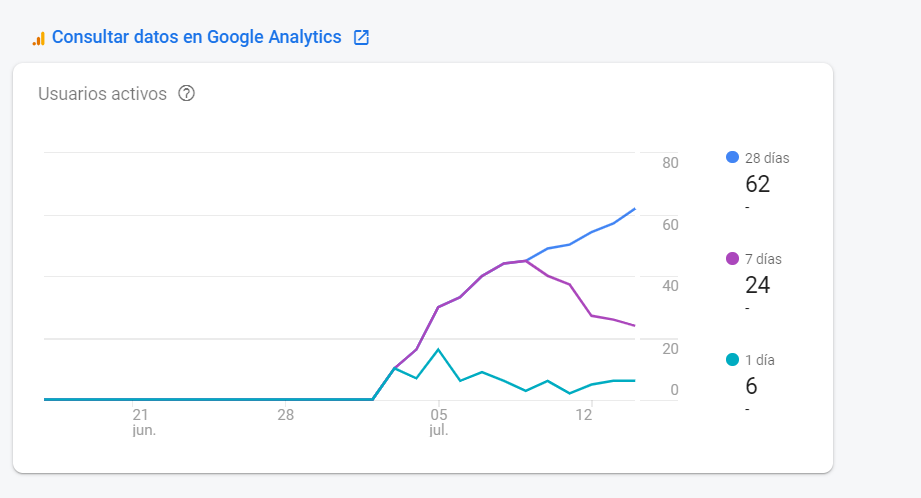
\includegraphics[width=1\textwidth]{teoria/numerousers.png}
		\caption{Ejemplo de Analytics}\label{fig:numerousers}
	\end{figure}
\end{itemize}
